\section{Testing del componente}
Il corretto funzionamento del componente è stato verificato tramite l'utilizzo dei test bench. Tre sono le modalità di simulazione eseguite: \textit{Behavioural}, \textit{Post-Synthesis Functional} e \textit{Post-Synthesis Timing}.\newline
A partire dai test bench di esempio, sono stati costruiti altri test bench che cercassero di simulare il maggior numero di possibili scenari d'esecuzione del modulo.\newline
Di seguito sono riportati i casi di test più significativi. I primi due forzano il controllo di tutte le working-zone presenti in RAM.

\begin{enumerate}

	\item \textbf{WZ MISS}: l'indirizzo da codificare non appartiene a nessuna working-zone.
	\begin{figure}[!htb]
		\centering
		%\setlength{\belowcaptionskip}{-0.5cm}
		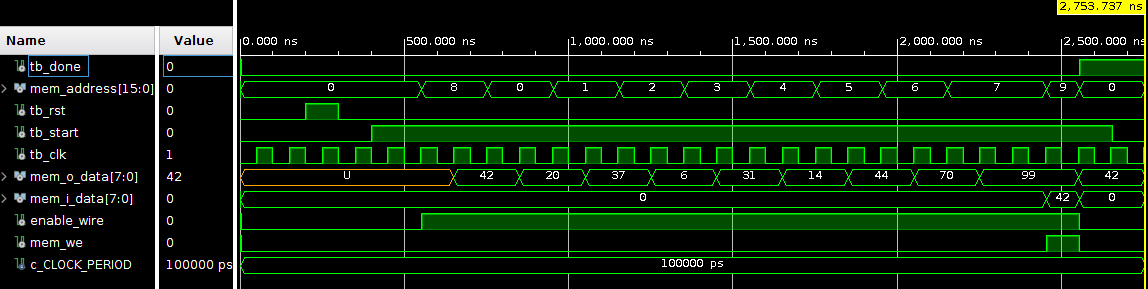
\includegraphics[scale=0.520]{images/wz_miss.png}
		\caption{waveform della simulazione con ADDR non appartenente a nessuna WZ.}
	\end{figure}
		
	\item \textbf{Ultima WZ HIT}: il test verifica la codifica dell'indirizzo nel caso in cui esso appartenga all'ultima working-zone disponibile in RAM (WZ 7).
	
	\item \textbf{Prima WZ HIT}: il test verifica la codifica dell'indirizzo nel caso in cui esso appartenga alla prima working-zone disponibile in RAM (WZ 0).
	\begin{figure}[!htb]
		%\setlength{\belowcaptionskip}{-0.5cm}
		\centering
		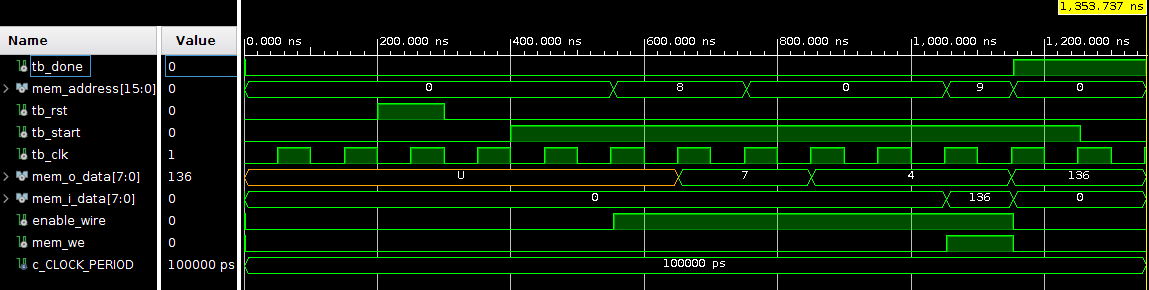
\includegraphics[scale=0.520]{images/first_wz_hit.png}
		\caption{waveform della simulazione con $ADDR=7$ appartenente alla prima WZ.}	
	\end{figure}

\end{enumerate}	

Ciascuno dei successivi test è stato eseguito sia in occorrenza \textit{\textbf{WZ MISS}} che \textit{\textbf{WZ HIT}}.

\begin{enumerate}[resume]
	
	\item \textbf{WZ adiacenti}: le working-zone caricate nella RAM sono una adiacente all'altra.
	
	\item \textbf{ADDR/WZ minimi}: l'indirizzo da codificare e/o una WZ corrispondono alla codifica in binario composta da soli zero "00000000" (0 in decimale).
	
	\item \textbf{ADDR massimo}: l'indirizzo da codificare corrisponde alla codifica in binario "01111111" (127 in decimale).
	
	\item \textbf{WZ massima}: l'indirizzo di una working-zone corrisponde alla codifica in binario "01111100" (124 in decimale). Questa rappresenta la massima codifica possibile su 8 bit (con il bit più significativo a 0) affinché la working-zone risulti completa, cioè con 4 indirizzi di offset (124, 125, 126, 127).

	\item \textbf{Reset asincrono}: il test verifica il comportamento della macchina quando il segnale di reset viene alzato in modo asincrono. La macchina torna nello stato di reset \texttt{IDLE} dove rimane in attesa di un nuovo segnale di inizio.
	\begin{figure}[!htb]
		\centering
		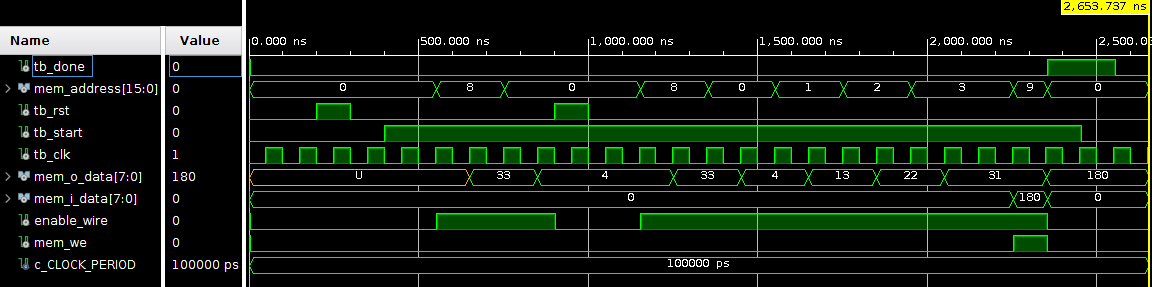
\includegraphics[scale=0.520]{images/async_reset.png}
		\caption{waveform della simulazione con reset asincrono.}	
	\end{figure}
	
	\item \textbf{Multi-start, stesse WZ}: il test effettua la codifica (in sequenza) di almeno due indirizzi diversi mantenendo invariate le working-zone durante ogni computazione.
	
	\item \textbf{Multi-start con reset (diverse WZ)}: il test effettua la codifica (in sequenza) di almeno due indirizzi. Le working-zone tra una computazione e l'altra vengono cambiate tramite l'asserzione del segnale \lstinline[columns=fixed]{i_rst}.
	
	\item \textbf{Frequenza elevata}: un caso di test è stato dedicato alla variazione della frequenza di elaborazione del modulo. Dal periodo di clock di default pari a 100ns si è testato fino ad un minimo di circa 5ns.
\end{enumerate}

Oltre ai test mirati proposti sopra, sfruttando la modalità batch di Vivado, sono stati si-mulati numerosi test bench generati casualmente da un apposito script scritto in Python.\newline
